\documentclass{article}

\usepackage{fullpage}
\usepackage{amsmath}
\usepackage{bm}
\usepackage{esdiff}
\usepackage{cite}
\usepackage{hyperref}
\usepackage{graphicx}

\renewcommand{\vec}[1]{\bm{\mathrm{#1}}}

\graphicspath{{./res/}}

\title{Kelvin-Helmoltz Instability}
\author{Jonathan Elsner}
\date{December 11\textsuperscript{th}, 2024}

\begin{document}

\maketitle

\section{Abstract}

% Maybe look at MIT guide to abstract writing?
Kelvin-Helmholtz (KH) instability is a process that occurs at the interface
between two fluids of two differing densities, creating vortex waves. KH
Instability is a commonly occurring process in nature: it is one of the driving
forces of mixing in the ocean \cite{woods-1968}, causes clear-air turbulence on
flights and can sometimes be seen in cloud formations \cite{ludlam-1967}. It is
also thought to be a factor in heating the corona of the Sun
\cite{nasa-solar-surfer}.

\begin{figure}[h]
    \centering
    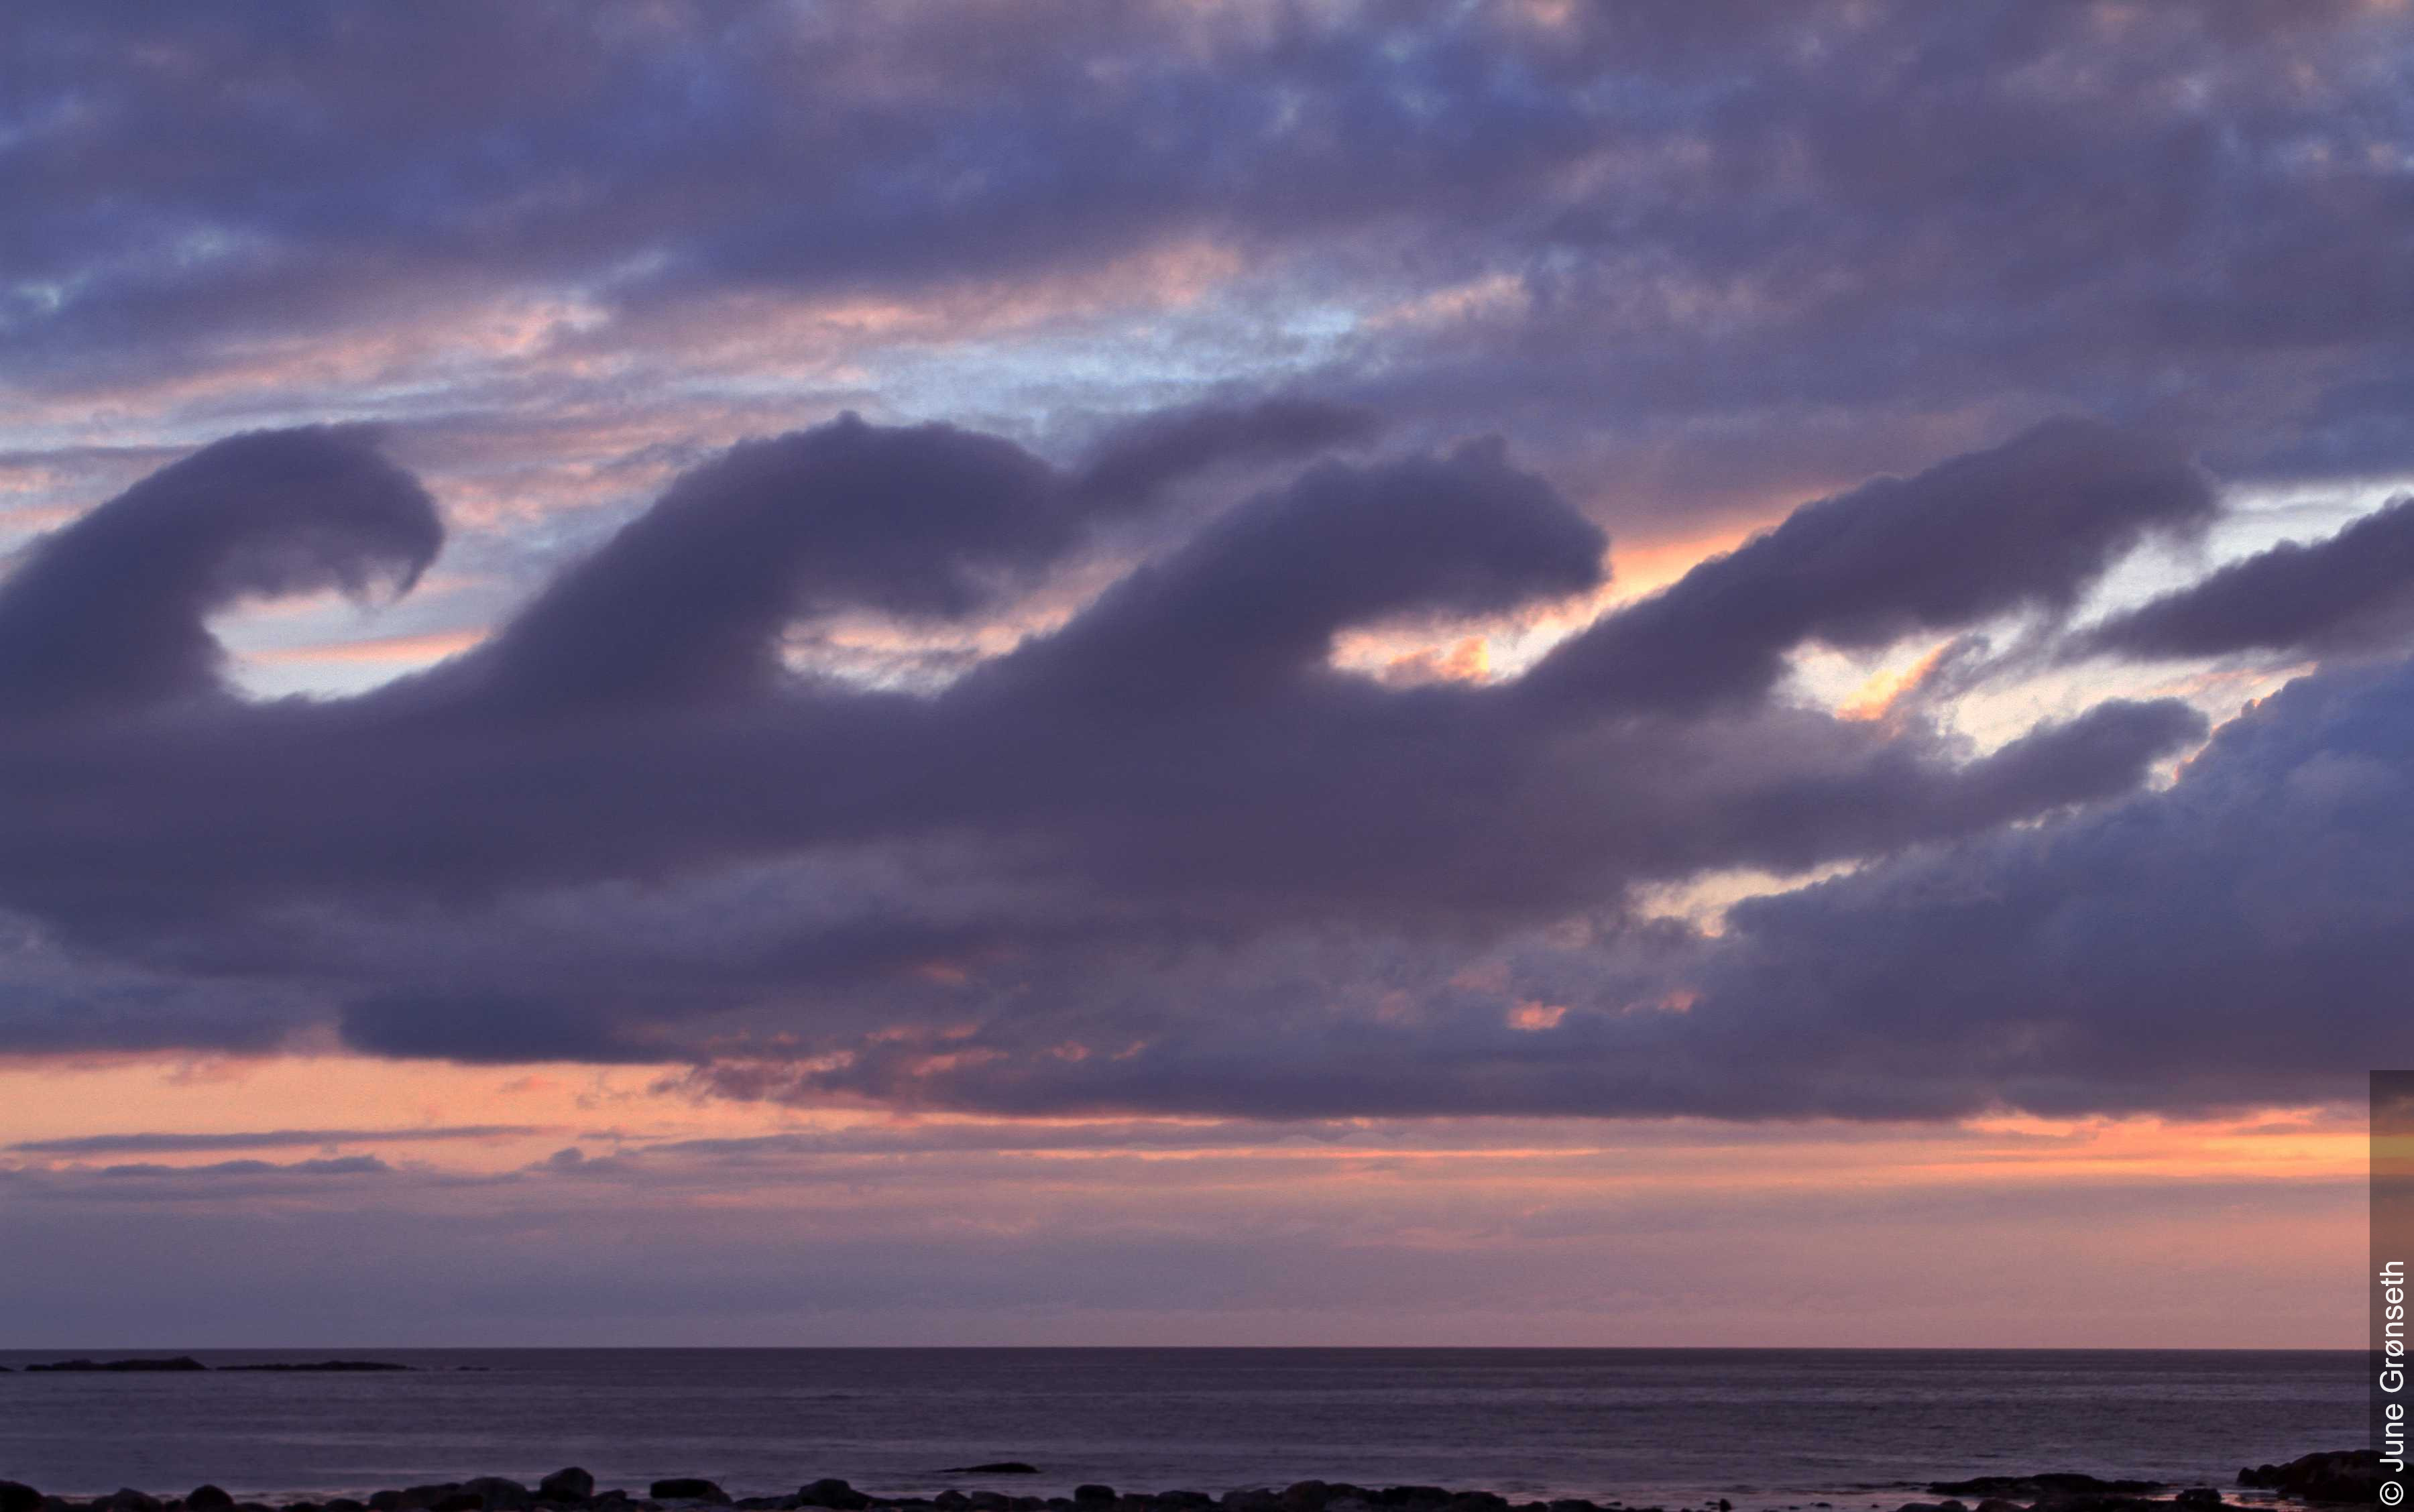
\includegraphics[width=4in]{kh-instability-clouds-2.jpg}
    \caption{Rare fluctus clouds are caused by KH Instability \cite{ludlam-1967}. Photo: \cite{fluctus-clouds}.}
    \label{img:fluctus-clouds}
\end{figure}

The key characteristic of KH instability is the distance between the waves at
the interface. This changes over time and is dependent on both the difference in
density between the fluids and the flow rate of each fluid \cite{kundu}.

We follow a procedure outlined in \cite{kh-instability-demo} to recreate this
phenomenon in the lab to analyze the results and determine the relationship
between fluid speed, fluid density, and instability wavelength. We also analyze
the evolution of the waves over time.
% Talk about findings?

\section{Procedure}

To carry out the experiment, we followed the following rough procedure, adopted
from \cite{kh-instability-demo}:

\begin{enumerate}
    \item Fill tank halfway with fresh water
    \item Mix salt for desired salinity. We calculated how much salt we wanted
    for a desired concentration, mixed that together, then verified the salinity
    with a handheld refractometer.
    \item Slowly fill the tank to full with the denser salt water.
    \item Return tank to level and allow the interface to stabilize
    \item Swiftly tilt tank to develop the instability.
\end{enumerate}

The denser fluid was dyed darkly to create a stark visual boundary between the
two fluids. We placed a light sheet behind the tank to form a uniform background
and consistently illuminate the fluid. We recorded video of the flow both on a
small scale in slow motion and at a wide angle capturing the entire tank.

We attempted to keep the rotation angle of the tank consistent by stopping the
rotation of the tank on a bucket placed under one end of the apparatus.

\section{Theory}

From Kundu \cite{kundu}, we model KH instability as the % FINISH!

Variables
\begin{itemize}
    \item \(U_1\): basic state velocity potential of the upper fluid.
    \item \(U_2 = -U_1\): basic state velocity potential of the lower fluid.
    \item \(\phi_1, \phi_2\): perturbation velocity potentials due to instability
    \item \(\tilde \phi_1, \tilde \phi_2\): total flow potentials
    \item \(\rho_1\): density of the upper fluid
    \item \(\rho_2 > \rho_1\): density of the lower fluid
    \item \(z = \zeta(x, t)\): height of the interface between the  fluids
\end{itemize}

Using Kelvin's circulation theorem, the flow is irrotational in the bulk of the
top and bottom fluids, hence the velocity potential in each half space must
satisfy the Laplacian:

\[ \nabla^2 \phi_i = 0\]

For \(i = 1, 2\).

Taking into account the boundary conditions:

\begin{itemize}
    \item \(\phi_1 = 0\) when \(z = L\)
    \item \(\phi_2 = 0\) when \(z = -L\)
    \item \(\vec n \cdot \nabla \tilde \phi_1 = \vec n \cdot \vec u_s = \vec n \cdot \nabla \phi_2\) on \(z = \zeta\)
    \item \(P_1 = P_2\) on \(z = \zeta\)
\end{itemize}
where \(\vec n(x, t)\) is the normal vector to the surface \(xi\), \(\vec u_s(x,
t)\) is its velocity (which is purely vertical), and \(P_1\) and \(P_2\) are the pressures above and below
the surface.

We can rewrite the interface boundary condition using unit vectors \(\vec e_x, \vec e_z\):

% good luck deciphering this
\[ \vec n \cdot \left[ \diffp{\tilde \phi_1}{x} \vec e_x + \diffp{\tilde \phi_1}{z} \vec e_z\right] = \vec n \cdot \left[ \diffp{\zeta}{t} \vec e_z\right] = \vec n \cdot \left[\diffp{\tilde \phi_2}{x} \vec e_x + \diffp{\tilde \phi_2}{z} \vec e_z \right]\]

Defining the normal vector using the implicit formula of a surface (\(f = z - \zeta = 0\)):
\[\vec n = \frac{z - \zeta(x, t)}{|z - \zeta(x, t)|} = \frac{\left(-\diffp{\zeta}{x}\right)\vec e_x + e_z}{\sqrt{1 + \left(\diffp{\zeta}{x}\right)^2}}\]

and using the fact that \(\vec u_s = \left(\diffp{\zeta}{t}\right)\vec e_z\), the condition simplifies to:

asdfasdf

\section{Results and Analysis}

Velocity data was not readily available from the videos of each run, so we
derived the velocity of each half of the tank using data on the height of the
interface. We used \href{https://physlets.org/tracker/}{Tracker} to extract the
motion of key components of the videos. We determined wave number by measuring
the distance between crests of the visible waves.

Fluid velocity was assumed to be equal and opposite for both sides of the fluid,
and determined by estimating the fluid flow. We measured the height of the
interface at both ends of the channel to calculate the volume of each liquid in
a defined space. To measure the height, we tracked the position of points on the
interface and the angle of the channel. We then transformed the positions so
that they were fixed relative to the tank; that is, we observed the positions
from a reference frame tracking the rotation of the channel.
\begin{figure}[h]
    \centering
    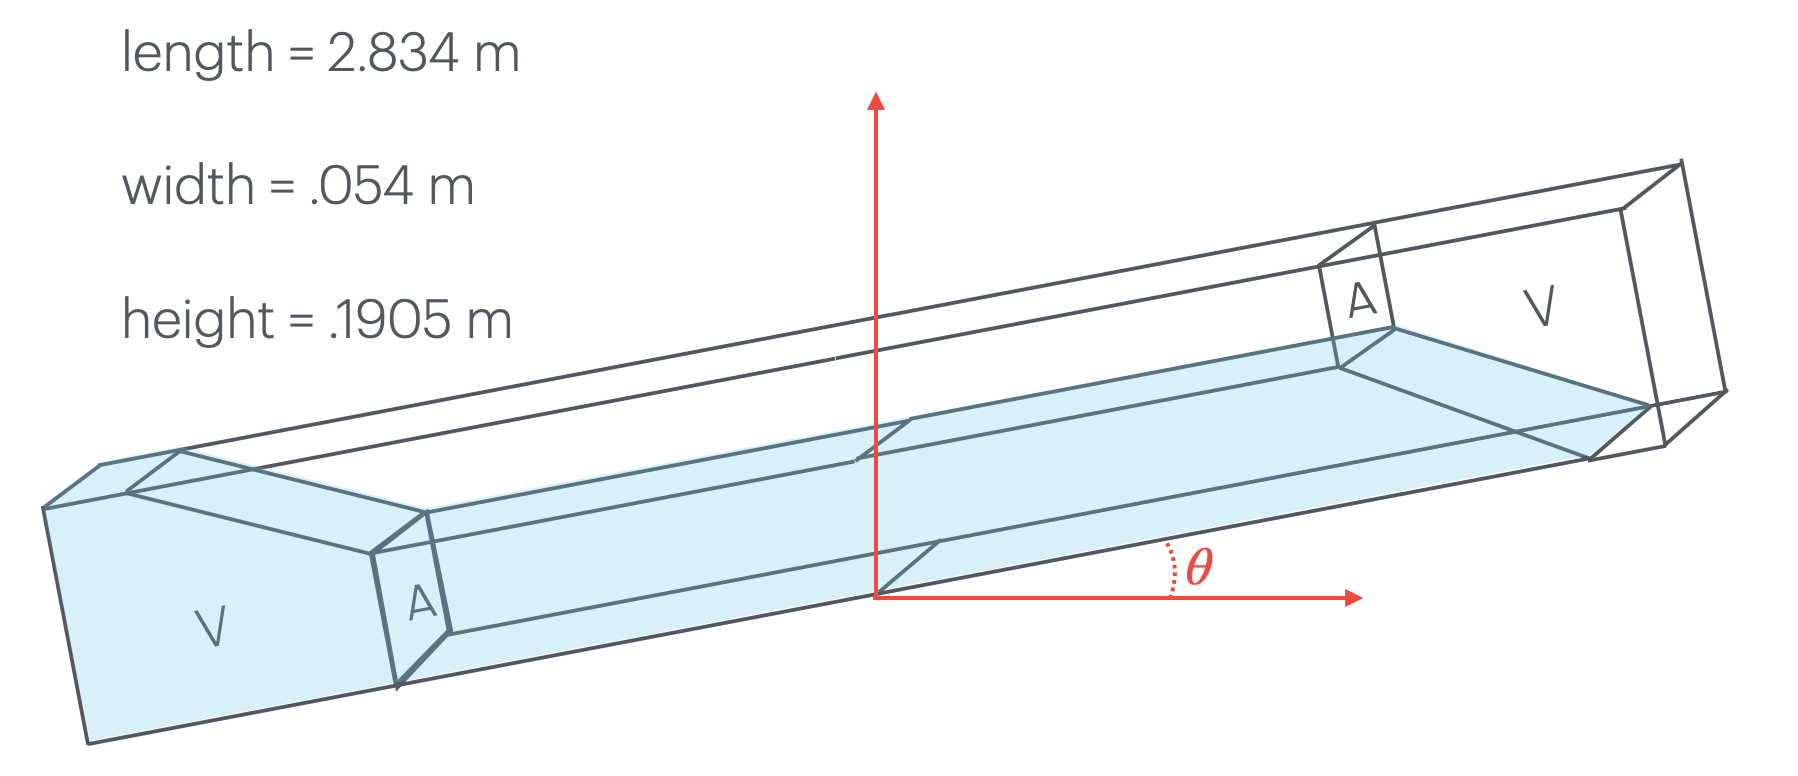
\includegraphics[width=5in]{tank-schematic.png}
    \caption{Schematic of the Tank. Coordinates were rotated by $-\theta$ so that the coordinate axes are parallel and perpendicular to the bottom of the channel.}
    \label{img:tank-schematic}
\end{figure}
Tracking the height
over time gives us the flow rate of the liquid, which we can divide by the cross
section of the channel to find the fluid velocity. The velocity varies over
time, so we chose to average the velocity during the time after the channel was
tilted, but before the instability started.

Using the density and fluid velocity, we can compute the Richardson number

\[ \text{Ri} = \frac{g}{\rho} \frac{\Delta \rho}{\Delta U} \]

where \(g\) is acceleration due to gravity and \(\rho\) is the density of one fluid, which we set to the density of fresh water (1000 kg/m\textsuperscript{2}) for this analysis.

\begin{table}[h!]
    \centering
    \begin{tabular}{|c|c|c|c|c|c|}
    \hline
    \textbf{Salinity (\%)} & $\bm{\Delta \rho}$ \textbf{(kg/m\textsuperscript{3})} & $\bm{\Delta U}$ \textbf{(m/s)}& \textbf{Ri} & $\bm{k}$ \textbf{(1/m)}& $\bm{\lambda}$ \textbf{(m)}\\ \hline
    3.5 & 24.640773 & 0.07 & 48.096414 & 43.744532 & 0.02286 \\ \hline
    9.5 & 70.584422 & 0.10 & 64.612124 & 56.242970 & 0.01778 \\ \hline
    15.0 & 112.699310 & 0.12 & 68.929800 & 65.616798 & 0.01524 \\ \hline
    \end{tabular}
    \caption{Summary of collected and derived data from the lab.}
    \label{tab:data}
\end{table}

In Figure \ref{graph:Ri-vs-k} we plot the relationship between Ri and \(k\).

\begin{figure}[h!]
    \centering
    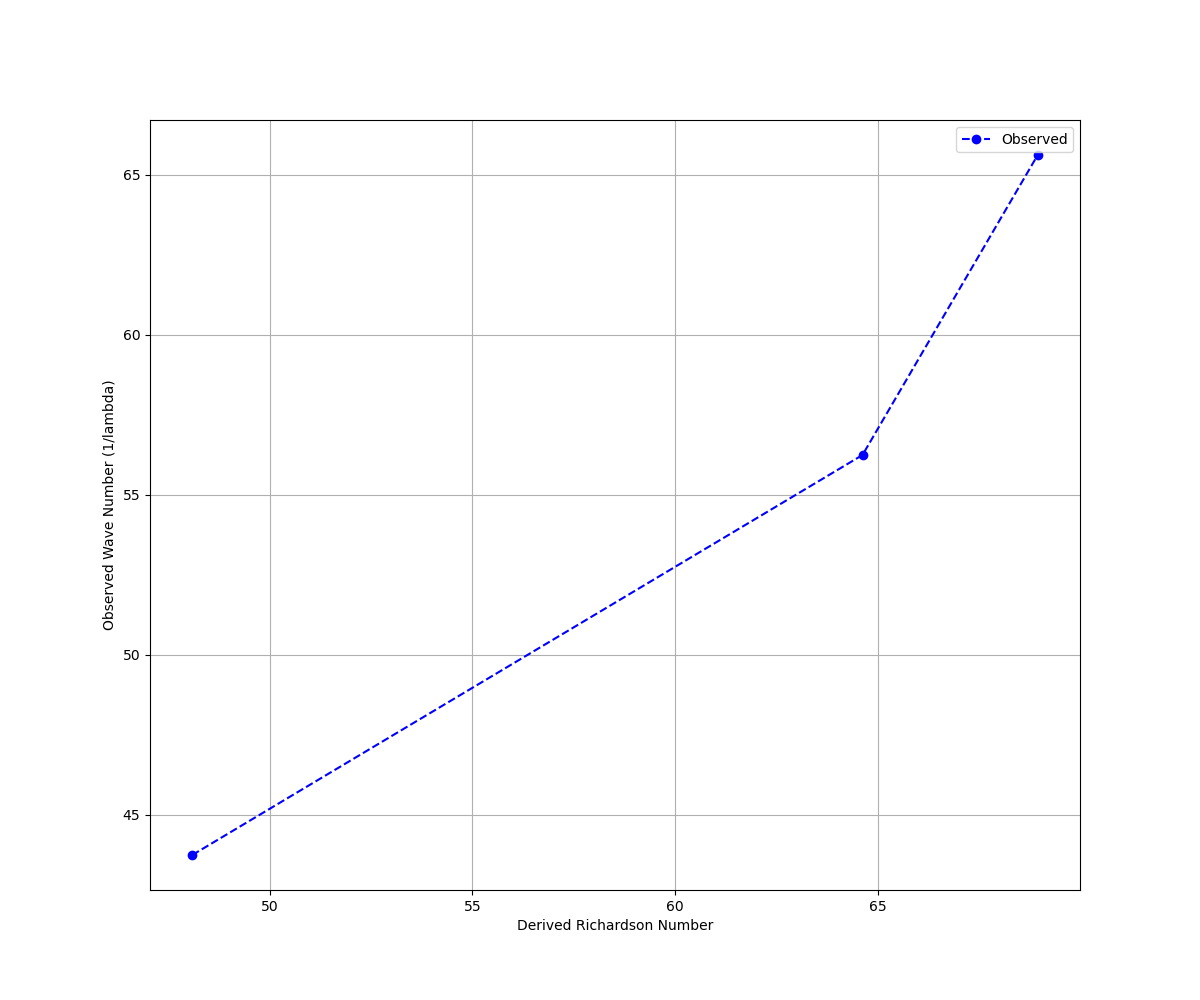
\includegraphics[width=5in]{RivsK.png}
    \caption{Wave number $k$ as a function of Ri. Admittedly, with three data points, it is hard to identify any kind of dependence.}
    \label{graph:Ri-vs-k}
\end{figure}

For Ri \(< 1/4\), we expect the system to remain 

\section{Future Work}

Several aspects of this experiment proved challenging. While it was relatively
easy (albeit time consuming) to create the phenomenon in a lab, collecting
useful data on the instability was harder. As a result, much post-processing had
to be done to produce useable data. Better planning and experimental design
would have mitigated these issues. In particular, we should have had a clear
idea of the independent and dependent variables at play before running the
experiment, in order collect relevant data for these variables. A clear,
unobstructed video recording of the entire tank is recommended in any future
research. Further, consistency of parameters between trials is important. This
includes camera placement, degree of tank tilt, and speed of tank tilt.
Maintaining solid control variables will ensure that multiple trials can be
easily compared.

\section{Acknowledgements}

We would like to thank the members of our group: Jesse Akes, Anna Dodson, and
Maddy Kovaleski. They were instrumental in making this project happen; it truly
was a team effort. Beyond the project, Jesse and Maddy provided immense support
this quarter, both academically and socially. We would also like to thank Georgy
Manucharyan and Noah Rosenberg for creating a welcoming, low-pressure
environment in class and teaching us a lot.  

\newpage
\bibliography{bibliography}{}
\bibliographystyle{plain}

\end{document}